%
% elliptisch.tex
%
% (c) 2008 Prof Dr Andreas Mueller
% $Id: c04-elliptisch.tex,v 1.3 2008/10/31 08:04:16 afm Exp $
%
\chapter{Elliptische Differentialgleichungen\label{chapter-elliptisch}}
\index{Differentialgleichung!partielle!elliptische}
\lhead{Elliptische PDGL}
In diesem Kapitel untersuchen wir L"osungen elliptischer Differentialgleichungen
und entdecken dabei die Mittelwerteigenschaft
harmonischer Funktionen sowie die Greensche Funktion, mit der sich f"ur
die L"osung des Randwertproblems eine Formel aufstellen l"asst.
\index{Mittelwerteigenschaft}
\index{Greensche Funktion}

\section{Einf"uhrung}
\rhead{Einf"uhrung}
In den bisherigen Kapiteln waren die Differentialgleichungen auf sehr
speziellen Gebieten definiert gewesen, zum Beispiel Rechtecken, Kreissscheiben,
unendlichen Streifen, Halbebenen oder auf ganz $\mathbb R^n$. 
Die Anwendungen verlangen aber, dass elliptische partielle
Differentialgleichungen, auf fast beliebigen Gebieten gel"ost werden k"onnen.
Insbesondere wollen wir erstehen, unter welchen Bedingungen eine
L"osung existiert und eindeutig bestimmt ist.

\subsection{Laplace-Gleichung}
\index{Laplace-Gleichung}
Als Beispiel f"ur die Eigenschaften der L"osungen
%\marginpar{\tiny Formulierung des Beispielproblems}
elliptischer linearer partieller Differentialgleichungen
betrachten wir in diesem Kapitel die Laplace-Gleichung
auf einem Gebiet $\Omega\subset\mathbb R^n$
\begin{equation}
\Delta u=f
\label{laplaceequation}
\end{equation}
mit
Dirichlet Randbedingungen
\begin{equation}
u_{|\partial \Omega}=g,
\label{dirichletrandbedingung}
\end{equation}
Neumann Randbedingungen
\[
\frac{\partial u}{\partial n}_{|\partial \Omega}=g
\]
oder der gemischten Randbedingungen
\[
\alpha u_{|\partial \Omega}+
\beta\frac{\partial u}{\partial n}_{|\partial \Omega}=g.
\]
Eine L"osung dieses Problems ist eine auf $\Omega$
zweimal stetig differenzierbare
Funktion $u$, welche stetig auf den Rand ausgedehnt werden kann,
und dort die Randbedingungen erf"ullt. Zur Vereinfachung der
Diskussion betrachten wir in diesem Abschnitt nur die
Dirichlet-Randbedingungen (\ref{dirichletrandbedingung}).

Aus der allgemeinen Theorie linearer partieller Differentialgleichungen
%\marginpar{\tiny Allgemeine L"osungsstrategie}
kann man ableiten, dass wir f"ur
die L"osung des gestellten Problems wie folgt vorgehen m"ussen
\begin{enumerate}
\item Zun"achst brauchen wir eine partikul"are
L"osung $u_p$ der Laplace-Gleichung (\ref{laplaceequation}).
\item Mit $u_p$ reduziert sich das Problem darauf, eine L"osung
$u_h=u-u_p$ der homogenen Gleichung $\Delta u_h=0$
zu finden, welche die Randbedingung
\[
u_{|\partial\Omega}=g-{u_p}_{|\partial\Omega}
\]
erf"ullt.
\item
Weitere L"osungen des Problems unterscheiden sich von dem
bereits gefundenen Problem nur durch eine Funktion $v$, welche
$\Delta v=0$ und $v_{|\partial\Omega}=0$ erf"ullt.
\end{enumerate}
Wir werden in diesem Kapitel zeigen, dass die L"osung diese Problems
eindeutig ist, dass also das einzige m"ogliche $v=0$ ist.
Ausserdem werden wir Formeln f"ur partikul"are L"osungen wie auch f"ur
das homogene Problem aufstellen.

\subsection{Harmonische Funktionen}
\index{harmonische Funktion}
Angesichts der Bedeutung der L"osungen des homogenen Problems
geben wir diesen einen speziellen Namen:

\begin{definition}
Eine zweimal stetig differenzierbare Funktion $u$ auf dem Gebiet $\Omega$
heisst harmonisch, wenn $\Delta u=0$.
\end{definition}

\section{Eindeutigkeit der L"osung}
Wir untersuchen jetzt die Frage, ob die L"osung des 
Dirichlet-Problems (\ref{laplaceequation}) und
(\ref{dirichletrandbedingung}), sollte sie existieren, eindeutig ist.
Seien also $u_1$ und $u_2$ zwei L"osungen des Problems. Die Differenz
$u=u_1-u_2$ erf"ullt dann
\begin{align*}
\Delta u&=\Delta u_1-\Delta u_2=f-f=0\\
u_{|\partial\Omega}&=u_{1|\partial\Omega}-u_{2|\partial\Omega}=g-g=0.
\end{align*}
$u$ ist also eine L"osung des homogenen Problems mit homogenen
Randbedingungen.

Diese Beobachtung trifft nat"urlich auch zu f"ur jeden anderen
Differentialoperator der Form
\[
L=\sum_{i,j}a_{ij}\partial_i\partial_j+\sum_i b_i\partial_i.
\]
Um die Eindeutigkeit der L"osung zu verstehen, muss man also verstehen,
ob das homogene Problem mit homogenen Randbedingungen eine
eindeutige L"osung hat. Dies wiederum folgt aus dem folgenden Satz.

\begin{satz}[Maximum-Prinzip f"ur elliptische Operatoren]
\label{maximumprinzip}
Ist $L$ ein elliptischer Differentialoperator auf einem zusammenh"angenden
und beschr"ankten Gebiet $\Omega$,
und $u$ eine L"osung von $Lu=0$,
dann nimmt $u$ sein Maximum und Minimum auf dem Rand an.
\end{satz}

Die Bedingung, dass das Gebiet $\Omega$ beschr"ankt sein muss, ist
wesentlich.
Die Funktion $u(x,y)=x$ ist harmonisch, $\Delta x=0$, und auf
dem Rand des Gebietes $\Omega=\{(x,y)\,|\,x>0\}$, n"amlich
der $y$-Achse nimmt, gilt $u(0,y)=0$.
Es gibt also mehr als eine L"osung des Dirichletproblems mit
homogenen Randbedingungen f"ur dieses Gebiet.

Auch der Zusammenhang des Gebietes ist wesentlich.  Definieren wir
die Funktion 
\[
u(x)=n\qquad\text{f"ur $2^{-n} < x < \frac{3}{2}2^{-n}$},
\]
dann ist $\Delta u=0$, da aber die Werte von $u$ unbeschr"ankt sind,
wird auch kein Maximum angenommen.

\begin{proof}[Beweisidee]
Wir f"uhren den Beweis mit Hilfe eines Widerspruchs. Wir nehmen
an, $u$ nehme in einem inneren Punkt $x$ des Gebietes $\Omega$ ein
Maximum an.

Wir d"urfen annehmen, dass die Matrix $a_{ij}$ diagonal ist,
und dass,
da $L$ elliptisch ist, die Diagonalelement $a_{ii}=\lambda_i$
alle positiv sind. Da das Maximum in $x$ angenommen wird, muss
mindestens eine zweite Ableitungen negativ sein:
\[
\frac{\partial^2u}{\partial x_i^2}
\le 0
\quad
\Rightarrow
\quad
\sum_{i}\lambda_i \frac{\partial^2u}{\partial x_i^2} \le 0
\quad
\Rightarrow
\quad
Lu<0
\]
Der Widerspruch zeigt, dass es kein inneres Maximum geben kann.

Dies ist jedoch kein Beweis, weil es keinen Grund gibt, warum
nicht alle zweiten Ableitungen von $u$ im Punkt $x$ verschwinden
k"onnten. Wir geben einen vollst"andigen Beweis am Ende dieses
Abschnittes.
\end{proof}

\begin{satz}
Es gibt h"ochstens eine L"osung der Gleichung
$Lu=f$ 
mit Randbedingung
$u_{|\partial\Omega}=g$.
\end{satz}

\begin{proof}[Beweis]
Seien $u_1$ und $u_2$ L"osungen, dann ist $u=u_1-u_2$ eine L"osung 
von $Lu=0$ mit Randbedingungen $u_{|\partial\Omega}=0$. Nach Satz
\ref{maximumprinzip} nimmt $u$ sein Maximum und sein Minimum auf dem Rand an,
es gilt
also $0\le u\le 0$ in ganz $\Omega$.
Daher ist $u=0$ oder $u_1=u-2$,
zwei verschiedene L"osungen kann es also nicht geben.
\end{proof}

{\small
\subsubsection{Ein Beweis des Maximum-Prinzips}
Im Folgenden wollen wir wie versprochen einen vollst"andigen Beweis f"ur das
Maximumprinzip angeben. Der wesentliche Punkt in der Beweisidee
war, dass $Lu=0$, wir aber bei einem Maximum (inkorrekterweise)
auf $Lu<0$ schliessen wollten. Dabei erlaubt unsere Method nur zu
schliessen, dass $Lu\le 0$.
Unser Argument beweist also nur die folgende Aussage:
\begin{satz}
\label{maximumgt}
Ist $L$ ein elliptischer Differentialoperator auf einem zusammenh"angenden
und beschr"ankten Gebiet $\Omega$,
und $u$ eine Funktion mit der Eigenschaft $Lu>0$,
dann nimmt $u$ sein Maximum auf dem Rand an.
\end{satz}

Daraus kann man jetzt aber auch folgern:
\begin{satz}
Ist $L$ ein elliptischer Differentialoperator auf einem zusammenh"angenden
und beschr"ankten Gebiet $\Omega$,
und $u$ eine Funktion mit der Eigenschaft $Lu\ge0$,
dann nimmt $u$ sein Maximum auf dem Rand an.
\end{satz}

\begin{proof}[Beweis]
Wir d"urfen wie in der bereits oben skizzierten Beweisidee annehmen,
dass im betrachteten Punkt $x$ die Koeffizientenmatrix $(a_{ij})$
diagonal ist und alle $a_{11}$ positiv sind.

Wir betrachten die Funktion $u_{\varepsilon}=u-\varepsilon e^{\lambda x_1}$.
Es gilt
\begin{align*}
Lu_{\varepsilon}&=Lu-\varepsilon L(e^{\lambda x_1})\\
&=Lu-\varepsilon(a_{11}\lambda^2+b_1\lambda)e^{\lambda x_1}
\end{align*}
Da $a_{11}>0$ gilt, wird das quadratische Polynom $a_{11}\lambda^2+b_1\lambda$
f"ur gen"ugend grosses $\lambda$ positiv, und damit 
\[
Lu_{\varepsilon}= Lu-\varepsilon(a_{11}\lambda^2+b_1\lambda)e^{\lambda x_1}<0
\]
f"ur jedes beliebige $\varepsilon$. Nach Satz \ref{maximumgt} wird das Maximum
von $u_\varepsilon$ also auf dem Rand angenommen.
Im Grenz"ubergang $\varepsilon\to 0$ ist $u^\varepsilon\to u$, also
muss auch $u$ das Maximum auf dem Rand annehmen.
\end{proof}

Setzt man $-u$ in den eben bewiesenen Satz, folgt das Minimumprinzip:
\index{Minimumprinzip}
\begin{satz}
Ist $L$ ein elliptischer Differentialoperator auf einem zusammenh"angenden
und beschr"ankten Gebiet $\Omega$,
und $u$ eine Funktion mit der Eigenschaft $Lu\le0$,
dann nimmt $u$ sein Maximum auf dem Rand an.
\end{satz}

F"ur L"osungen von $Lu=0$ folgt dann der Satz \ref{maximumprinzip}.
}

\section{Gibt es einen zu $\Delta$ inversen Operator?}
Um das Problem $\Delta u=f$ zu l"osen, m"usste man einfach einen
inversen Operator $\Delta^{-1}$ kennen, dann w"are die gesuchte
L"osung $u=\Delta^{-1}f$. Dies ist nat"urlich zu sch"on, um wahr
zu sein, aber die folgenden zwei Beispiele sollen illustrieren,
dass f"ur elliptische Operatoren
mindestens etwas "Ahnliches durchaus im Bereich des M"oglichen
liegen k"onnte.

\subsection{Ableitung und Integration}
Die Gleichung in einer Dimension
\[
u''(x)=f(x)
\]
kann direkt mit Hilfe von Integrationen gel"ost werden. Dazu muss
man nur eine Stammfunktion $F$ von $f$ finden, also $F' = f$ und
weiter eine Stammfunktion $u$ von $F$, dann gilt
$u''(x)=F'(x)=f(x)$. Trotzdem ist $u$ noch keine L"osung, denn 
sie erf"ullt die Randbedingungen noch nicht.

\subsection{Lineare Gleichungen}
Man kann sich vorstellen, dass durch Diskretisation aus der 
Differentialgleichung $u''=f$ auf dem Interval $[a,b]$ ein lineares Gleichungssystem
$Au=f$ entsteht. Die Komponenten der Vektoren $u$ und $f$ sind dabei
Werte von $u$ und $f$ an ausgew"ahlten Punkten. Und es ist nicht
abwegig, dass es eine inverse Matrix $G$ geben k"onnte, mit der man
die L"osung $u=Gf$ finden k"onnte.

Das Matrizenprodukt ist
\[
\sum_{j}g_{ij}f_j = u_i,
\]
und auch die $g_{ij}$ k"onnte man als Werte einer Funktion $G(x,y)$
betrachten. Die Summe ist dann nur der diskrete Fall eines Integrals,
man k"onnte also auf die Idee kommen, dass
die L"osung $u$ mit einer Formel der Form
\[
u(x)=\int_a^b G(x,\xi)f(\xi)\,d\xi
\]
gefunden werden kann. Auch dies wird noch nicht funktionieren,
weil wiederum die Randbedingung nicht ber"ucksichtigt wurde.

\subsection{Randbedingungen}
Die Randbedingungen sollten ebenfalls linear in das Problem eingehen.
Im eindimensionalen Problem haben wir nur zwei Punkte auf dem Rand,
also m"ussten sie einen Beitrag der Form
\[
K(x,a) g(a) + K(x,b)g(b)
\]
beitragen. Besteht der Rand dagegen aus vielen Punkten, w"urde dies
wieder zu einer grossen Summe
\[
\sum_{i}K(x,a_i)g(a_i),
\]
wobei die Punkte $a_i$ auf dem Rand liegen. In der Grenze erwartet man
als f"ur die Randwerte einen zweiten Beitrag
\[
\int_{\partial\Omega}K(x,\xi)g(\xi)\,d\xi
\]
in Form eines Kurven- oder Oberfl"achenintegrals "uber den Rand des
Gebietes.
Wir suchen daher eine allgmeine L"osung des Problems in der Form
\begin{equation}
u(x)=\int_{\Omega} G(x,\xi)f(\xi)\,d\xi + \int_{\partial\Omega} K(x,\xi)g(\xi)\,d\xi.
\label{greenformula}
\end{equation}

\section{Das eindimensionale Problem}
\rhead{Der eindimensionale Fall}
Zum Beweis, dass das im vorangegangenen Abschnitt angedeutete Programm 
tats"achlich durchf"uhrbar ist,
betrachten wird das eindimensionale Problem
\[
u''(x)=f(x)
\]
mit der Randbedingung
\[
u(0)=a,\quad u(1)=b.
\]
Ziel ist, die Funktion $G$ zu finden.

Die L"osung dieses Problems wird in der Theorie der gew"ohnlichen
%\marginpar{\tiny L"osung des gew"ohnlichen Randwertproblems als Leitlinie
%f"ur den mehrdimensionalen Fall}
Differential\-gleichungen behandelt, wir wollen hier die allgemeine
L"osung jedoch so darstellen, dass sie als Leitlinie f"ur die
Entwicklung einer L"osung f"ur das mehrdimensionale Problem dienen
kann.
\subsection{Partikul"are L"osung}
Ein L"osung der Gleichung kann sofort gefunden werden, die Stammfunktion
liefert die L"osung
\begin{align*}
u_p'(x)&=\int_0^xf(\xi)\,d\xi,
\\
u_p(x)&=\int_0^xu_p'(\eta)\,d\eta=\int_0^x\int_0^\eta f(\xi)\,d\xi\,d\eta
\end{align*}
diese erf"ullt aber die Randbedingung nicht.
Die gesuchte L"osung muss aber eine Summe der partikul"aren L"osung 
und einer L"osung der homogenen Gleichung
\[
u_p''(x) + u_h''(x)=f(x)\quad\Rightarrow\quad u_h''(x)=0
\]
sein, mit der Randbedingungen
\begin{align*}
u_h(0)&=a-u_p(0)=a\\
u_h(1)&=b-u_p(1)=b-\int_0^1\int_0^\eta f(\xi)\,d\xi\,d\eta
\end{align*}

\subsection{Das homogene Problem}
Das homogene Problem
\[
u''(x)=0
\]
kann mit den Standardverfahren gel"ost werden. Die allgemeine
L"osung hat die Form $Ax+B$, die Konstanten m"ussen so gew"ahlt werden,
dass die Randbedingungen erf"ullt sind, also
\begin{align*}
A\cdot 0+B&=a\qquad\Rightarrow&B&=a\\
A\cdot 1+B&=b\qquad\Rightarrow&A&=b-a
\end{align*}
also $u(x)=(b-a)x+a=(1-x)a+xb$.

\subsection{Allgemeine L"osung}
Im vorliegenden Fall sollte $u_h$ den rechten Randwert $b-\int_0^1\int_0^\eta f(\xi)\,d\xi\,d\eta$
annehmen, also
\[
u_h(x)=(1-x)a+x\left(b-\int_0^1\int_0^\eta f(\xi)\,d\xi\,d\eta\right).
\]
Damit wird die vollst"andige L"osung
\begin{align}
u(x)&=u_p(x)+u_h(x)\notag
\\
&=\int_0^x\int_0^\eta f(\xi)\,d\xi\,d\eta+(1-x)a+x\left(b-\int_0^1\int_0^\eta f(\xi)\,d\xi\,d\eta\right)\notag
\\
&=
(1-x)a+xb
+\int_0^x\int_0^\eta f(\xi)\,d\xi\,d\eta
-x\int_0^1\int_0^\eta f(\xi)\,d\xi\,d\eta\notag
\\
&=
(1-x)a+xb
+\int_0^1\vartheta(x-\eta)\int_0^1 \vartheta(\eta - \xi)f(\xi)\,d\xi\,d\eta
-x\int_0^1\int_0^1\vartheta(\eta-\xi) f(\xi)\,d\xi\,d\eta\notag
\\
&=
(1-x)a+xb
+\int_0^1\int_0^1
(\vartheta(x-\eta)-x)\vartheta(\eta -\xi)
f(\xi)\,d\xi\,d\eta
\notag
\\
&=
(1-x)a+xb+\int_0^1\int_0^1
(\vartheta(x-\eta)-x)\vartheta(\eta -\xi)
\,d\eta\,
f(\xi)\,d\xi
\label{1dimgreen}
\end{align}
Darin ist $\vartheta(t)$ die Stufenfunktion
\[
\vartheta(t)=\begin{cases}
0&\qquad t<0\\
1&\qquad t\ge 0
\end{cases}
\]
Die Funktion $\vartheta(x-\xi)$ verschwindet, sobald $\xi$ gr"osser wird
als $x$, da dann $x-\xi<0$ gilt.

Das innere Integral in (\ref{1dimgreen}) kann vollst"andig berechnet
werden:
\begin{align*}
\int_0^1(\vartheta(x-\eta)-x)\vartheta(\eta-\xi)\,d\eta
&=
\int_\xi^1\vartheta(x-\eta)-x\,d\eta
\\
&=
\int_\xi^1\vartheta(x-\eta)\,d\eta-\int_\xi^1x\,d\eta
\\
&=
\int_\xi^1\vartheta(x-\eta)\,d\eta-(1-\xi)x
\end{align*}
Das erste Integral muss mit einer Fallunterscheidung berechnet werden:
\begin{align*}
\int_\xi^1\vartheta(x-\eta)\,d\eta
&=
\begin{cases}
\int_\xi^x\,d\eta=x-\xi&\qquad\eta>\xi\\
0&\qquad x\le \xi
\end{cases}
\\
&=(x-\xi)\vartheta(x-\xi)
\end{align*}
Insgesamt finden wir also f"ur das innere
Integral die Funktion
\[
h(x,\xi)=(x-\xi)\vartheta(x-\xi)-x(1-\xi).
\]
Man kann diese Funktion auch mit Hilfe der Betragsfunktion
schreiben.
Die Funktion $x\mapsto h(x,\xi)$ ist an der Stelle $\xi$ nicht 
differenzierbar, links und rechts davon ist $h$ jedoch linear
\[
h(x,\xi)=\begin{cases}
(x-\xi)-x(1-\xi)=\xi(x-1)&\qquad x>\xi\\
x(\xi-1)&\qquad x<\xi
\end{cases}
\]
Also sollte in der Form $a|x-\xi|+bx+c$ geschrieben
werden k"onnen, nach etwas Rechnung findet man.
\[
h(x,\xi)={\textstyle \frac12}|x-\xi|-({\textstyle \frac12}-\xi)x-{\textstyle\frac12}\xi.
\]
Der zweite und dritte Term auf der rechten Seite bilden eine lineare
Funktion, die zur zweiten Ableitung nichts beitr"agt. Die Ableitung
des ersten Teils ist eine Stufenfunktion mit Stufenh"ohe $1$:
\[
\frac{\partial}{\partial x}({\textstyle \frac12}|x-\xi|)
=
\vartheta(x-\xi)
-
{\textstyle\frac12},
\]
und die Ableitung davon ist eine $\delta$-Funktion
\[
\frac{\partial^2}{\partial x^2}({\textstyle \frac12}|x-\xi|)
=
\delta(x-\xi).
\]
Der wesentliche Teil ist also die Funktion
\begin{equation}
\sigma(x,\xi)=\frac12|x-\xi|.\label{n1sigma}
\end{equation}

\subsection{Greensche Funktion}
\begin{figure}
\begin{center}
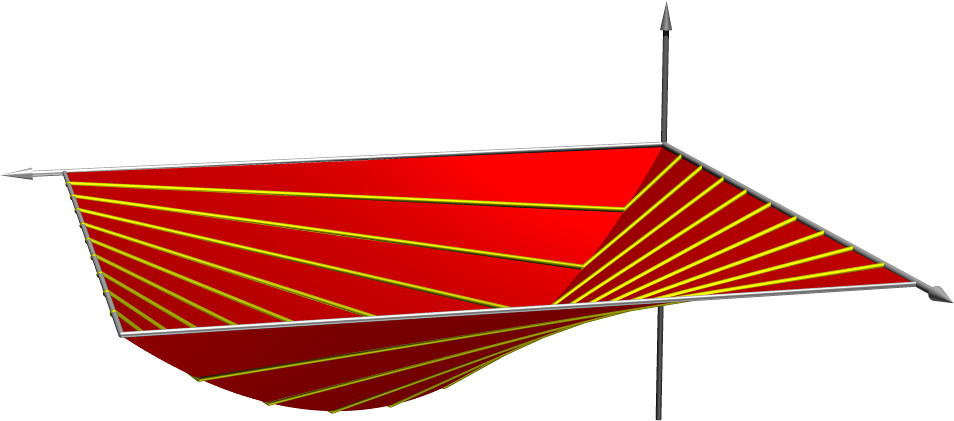
\includegraphics[width=\hsize]{3d/green.jpg}
\end{center}
\caption{Darstellung der Greenschen Funktion $G(x,\xi)$
f"ur das Problem $u''=f$ auf
dem Interval $[0,1]$ als Fl"ache "uber dem Quadrat $(x,\xi)\in[0,1]^2$.
F"ur jeden Wert von $\xi$ ist die partielle Funktion $x\mapsto G(x,\xi)$
eine L"osung der Differentialgleichung $u''=\delta_\xi$ zu den Randbedingungen
$u(0)=u(1)=0$.
\label{elliptisch:green3dflaeche}}
\end{figure}
\begin{figure}
\begin{center}
\includegraphics{images/green-1.pdf}
\end{center}
\caption{Partielle Funktionen $x\mapsto G(x,\xi)$ der Greensche Funktion
des Problems $u''=f$ mit Randbedingungen $u(0)=u(1)=0$ f"ur
verschiedene Werte von $\xi$.
\label{elliptisch:green1schar}}
\end{figure}

Die bis jetzt gefundenen Formeln f"ur die L"osung $u(x)$
in Form eines Doppelintegrals haben noch
nicht die gew"unschte Form eines einfachen Integrals.
Dies kann mit der Funktion $h$ korrigiert werden.
Die Funktion $x\mapsto h(x,\xi)=(x-\xi)\vartheta(x-\xi)$ hat die Randwerte
$0$ und $1-\xi$, also hat die Funktion
\[
G(x,\xi)=(x-\xi)\vartheta(x-\xi)-x(1-\xi)
\]
die Randwerte $0$.
$G$ erf"ullt
\[
\frac{\partial^2}{\partial x^2}G(x,\xi)=\delta(x-\xi)
\]
und
\[
G(0,\xi)=G(1,\xi)=0.
\]
Eine L"osung der Differentialgleichung l"asst sich damit
als 
\[
u(x)=\int_0^1G(x,\xi)f(\xi)\,d\xi+a(1-x)+bx
\]
finden.

Der eindimensionale Fall zeigt also, dass man man zu dem Operator $D^2u=f$
mit der Funktion $G$ eine Inverse konstruieren kann.

Die Abbildungen \ref{elliptisch:green3dflaeche} und
\ref{elliptisch:green1schar} zeigen die Greensche Funktion $G(x,\xi)$.
Die Partiellen Funktionen $x\mapsto G(x,\xi)$ sind jeweils L"osungen
des Problems $u''=\delta_\xi$ mit Randwerten $u(0)=u(1)=0$.
In den Abbildungen sind die partiellen Funktionen f"ur eine Anzahl
von Werten $\xi$ hervorgehoben.

\begin{beispiel}
Die Differentialgleichung
\[
y''=\cos 3\pi x.
\]
hat die L"osung
\[
y(x)=-\frac1{9\pi^2}(\cos 3\pi x + 2x - 1),
\]
die man auch mit der Greenschen Funktion berechnen kann:
\[
y(x)=\int_0^1 G(x,\xi)\cos 3\pi\xi\,d\xi.
\]
In Abbildung
\ref{elliptisch:green-beispiele}
ist $f(x)=\cos 3\pi x$ durch eine Summe von einigen $\delta$-Distribution
approximiert worden (blau).
Die zugeh"orige L"osung ist jeweils rot eingezeichnet, sie hat
Knicke bei den $\delta$-Funktionen. 
Bei gr"osser werdender Zahl von $\delta$-Funktionen unterscheidet sich
das Integral $\int G(x,\xi)f(\xi)\,d\xi$ kaum mehr von der L"osung.
\begin{figure}
\begin{center}
\includegraphics[width=0.7\hsize]{graphics/green-1.pdf}\\
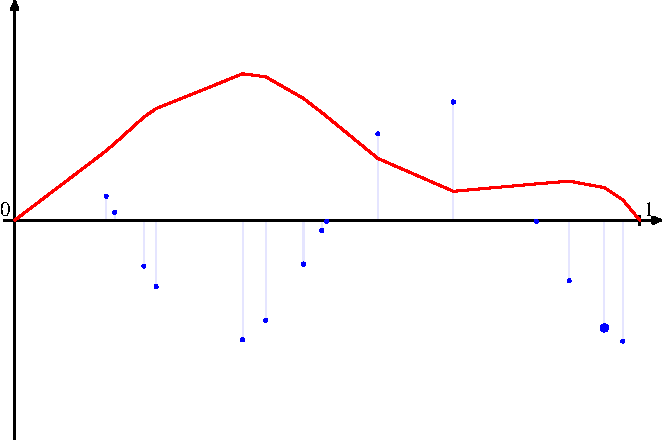
\includegraphics[width=0.7\hsize]{graphics/green-324.pdf}\\
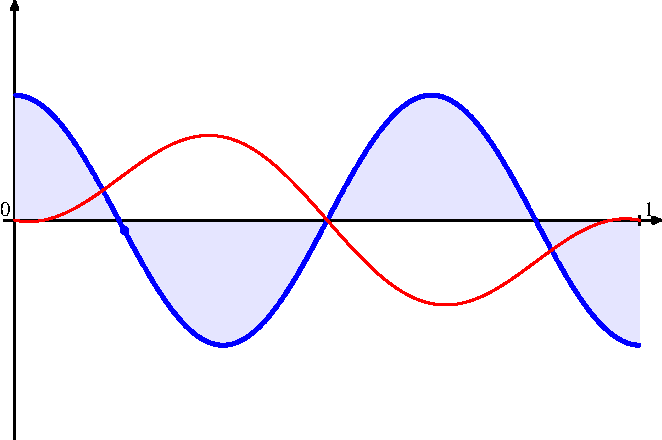
\includegraphics[width=0.7\hsize]{graphics/green-1082.pdf}
\end{center}
\caption{L"osung (rot) von $y''=f$ f"ur die Approximation der Funktion $f$
durch eine Summe von $\delta$-Distributionen (blau).
\label{elliptisch:green-beispiele}}
\end{figure}

Eine Animation der Berechnung der L"osung $y(x)$ mit der Greenschen
Funktion ist auch auf Youtube zu finden: \url{http://www.youtube.com/watch?v=Wpi7Gf7V2HY}
\end{beispiel}

\section{Der allgemeine Fall}
Wir m"ochten jetzt den allgemeinen Fall des Problems
\begin{align*}
\Delta u&=f&&\text{in $\Omega$}\\
u&=g&&\text{auf $\partial\Omega$}
\end{align*}
mit Hilfe einer Integralformel der Art (\ref{greenformula}) 
l"osen. Nach dem Muster des eindimensionalen Falles suchen
wir eine partikul"are L"osung $G(x,\xi)$ f"ur eine spezielle rechte Seite,
n"amlich eine Delta-Funktion im Punkt $\xi$.  Hat man eine
solche, kann man auch die L"osung f"ur ein beliebiges $f$ mit
Hilfe eines Integrals finden.


\subsection{Eine partikul"are L"osung}
\rhead{Partikul"are L"osung}
Das eindimensionale Musterproblem suggeriert, dass es eine
Funktion $\sigma(x,\xi)$ gibt, mit welcher eine partikul"are L"osung
der Laplace-Gleichung mittels des Integrals
\begin{equation}
u_p(x)=\int_\Omega \sigma(x,\xi)  f(\xi)\,d\xi
\label{singulaereloesunglaplace}
\end{equation}
gefunden werden kann.
Diese partikul"are L"osung muss die Randbedingungen nicht erf"ullen,
sondern nur die Gleichung $\Delta u=f$.

Die Funktion $\sigma$ h"angt, da sie auf die Randbedingungen nicht 
R"ucksicht nehmen muss, nicht von $\Omega$ ab, sondern nur von der
Dimension $n$.
W"ahlt man f"ur $f$ eine $\delta$-Funktion im Punkt $y$, folgt
\[
u(x)
=
\int_\Omega \sigma(x,\xi)\delta(\xi - y)\,d\xi
=
\sigma(x,y).
\]
Die Funktion $x\mapsto \sigma(x,y)$ erf"ullt also die Gleichung
$\Delta \sigma(x,y)=0$ f"ur alle Punkte von ${\mathbb R}^n\setminus\{y\}$.
Die Funktion $\sigma$ muss also eine harmonische Funktion in 
$\mathbb R^n\setminus\{y\}$ sein.

Die Bestimmung der Funktionen $\sigma(x,y)$ ist etwas m"uhsam, und wir
geben hier nur das Resultat an.
Man findet,\footnote{Man kann
diese L"osungen mit folgendem Argument finden. Zun"achst darf die L"osung
nur von der Entfernung $|x-\xi|$ abh"angen, so dass wir ohne
Beschr"ankung der Allgemeinheit $\xi=0$ annehmen d"urfen.
Da $\Delta u=\operatorname{div}\operatorname{grad}u$ gilt folgt mit
dem Satz von Gauss
\begin{align*}
1&=\int_{B_r^n} \Delta u(x)\,d\mu(x)
=
\int_{B_r^n} \operatorname{div}\operatorname{grad} u(x)\,d\mu(x)
=\int_{S_r^{n-1}}\operatorname{grad}u(x)\cdot dn
\\
&=\int_{S_r^{n-1}}|\operatorname{grad}u(x)|\,d\mu(x)
=\mu(S_r^{n-1})\left|\frac{d}{dr}u(r)\right|
\\
\Rightarrow\qquad\frac{d}{dr}u(r)
&=\frac1{\mu(S_r^{n-1})}
=\frac1{\mu(S_1^{n-1})r^{n-1}}.
\end{align*}
F"ur $n=2$ ist $\mu(S_r^1)=2\pi r$, also
\[
u'(r)=\frac1{2\pi r}\quad\Rightarrow\quad u(r)=\frac1{2\pi}\log|r|.
\]
F"ur $n\ge 3$ gilt
\[
u'(r)=\frac1{\mu(S^{n-1})}r^{1-n}\quad\Rightarrow\quad u(r)=\frac1{\mu(S^{n-1})}\cdot \frac1{2-n}r^{2-n}.
\]
} und f"ur $n=1$ haben wir diese Funktion ja schon in (\ref{n1sigma})
gefunden,
als L"osung
\begin{equation}
\sigma(x,\xi)=
\begin{cases}
\displaystyle \frac12|x-\xi|
&\qquad \text{f"ur $n=1$}
\\
\\
\displaystyle \frac1{2\pi}\log|x-\xi]
&\qquad \text{f"ur $n=2$}
\\
\\
\displaystyle -\frac1{4\pi}\frac1{|x-\xi|}
&\qquad \text{f"ur $n= 3$}
\\
\\
\displaystyle \frac1{(2-n)\mu(S^{n-1})}|x-\xi|^{2-n}
&\qquad \text{f"ur $n\ge 3$}
\end{cases}
\end{equation}
Durch etwas langweiliges Ausrechnen der Ableitungen kann man verifizieren,
dass diese Funktionen tats"achlich L"osungen sind, und dass
(\ref{singulaereloesunglaplace}) eine partikul"are L"osung der
Laplace-Gleichung ist.

\subsection{Greensche Funktion}
\rhead{Greensche Funktion}
Die vorgeschlagenen $\sigma$ sind nicht die einzigen f"ur die die
Formel (\ref{singulaereloesunglaplace}) eine partikul"are L"osung ergibt.
Addiert man zu $\sigma$ eine beliebige Funktion $h(x,\xi)$, die
also Funktion von $x$ harmonisch ist, dann ist
\[
u(x)=\int_{\Omega}\sigma(x,\xi)f(\xi)\,d\xi+\int_{\Omega}h(x,\xi)f(\xi)\,d\xi
\]
ebenfalls eine L"osung von (\ref{laplaceequation}). Insbesondere
k"onnten wir $h(x,\xi)$ so w"ahlen, dass
$x\mapsto h(x,\xi)$ eine L"osung des Randwertproblems
\begin{align*}
\Delta_x h(x,\xi)&=0&&x\in\Omega\\
h(x,\xi)&=-\sigma(x,\xi)&&x\in\partial\Omega
\end{align*}
ist. Dann ist $\sigma(x,\xi)+h(x,\xi)$ eine Funktion, die auf dem
Rand $\partial\Omega$ immer verschwindet. Die mittels
(\ref{singulaereloesunglaplace}) gefundene L"osung $u(x)$
verschwindet ebenfalls auf dem Rand.
%\marginpar{\tiny Greensche Funktion f"ur das Dirichletproblem auf $\Omega$}
Wir bezeichnen $\sigma+h$ f"ur diese spezielle Wahl von $h$ mit
\[
G(x,\xi)=\sigma(x,\xi)+h(x,\xi)
\]
und nennen sie die Greensche Funktion f"ur das Dirichlet Problem.

\begin{satz}Ist $\Omega$ ein Gebiet, auf dem das Dirichlet-Problem
eindeutig l"osbar ist, dann gibt es eine 
Funktion $G(x,\xi)$,
welche als Funktion von $x$ die Gleichung
\[
\Delta G(x,\xi)=\delta(x-\xi)
\]
l"ost mit homogenen Randbedingungen.
\end{satz}

Man beachte, dass dieser Satz zwar die Existenz einer Greenschen Funktion
garantiert, aber keinen Hinweis gibt, wie sie berechnet werden kann.
Die Greensche Funktion h"angt aber nur vom Gebiet ab, nicht von den
Randbedingungen.
Da es Gebiete gibt, auf denen das Dirichlet-Problem nicht ohne zus"atzliche
Veraussetzungen eindeutig l"osbar ist (siehe "Ubungen), ist die
Vorassetzung an das Gebiet notwendig.

Die Greensche Funktion l"ost aber nicht nur das Dirichlet-Problem
mit homogenen Randbedingungen ($g=0$), sondern "uberhaupt
unser Problem:

\begin{satz}[L"osung des Dirichlet-Problems]
\label{dirichletloesung}
Ist $G$ die Greensche Funktion f"ur das Dirichlet-Problem auf dem
%\marginpar{\tiny Greensche Funktion l"ost das Dirichlet-Problem}
Gebiet $\Omega$, dann ist
\[
u(x)=\int_{\Omega}G(x,\xi)f(\xi)\,d\mu(\xi)+\int_{\partial\Omega}g(\xi)\operatorname{grad}_\xi G(x,\xi)\cdot dn
\]
die L"osung des Dirichlet-Problems (\ref{laplaceequation}) und
(\ref{dirichletrandbedingung}).
\end{satz}


\begin{proof}[Beweis]
Wir wissen bereits, dass das Integral "uber $\Omega$ eine L"osung der
inhomogenen Gleichung mit homogenen Randbedingungen ist, es
bleibt also nur noch zu verstehen, dass das Integral "uber $\partial \Omega$
eine harmonische Funktion ist, welche die Randwerte $g$ hat.

F"ur diesen Beweis ben"otigen wir die folgende Identit"at
\begin{align*}
\operatorname{div}(u\operatorname{grad}v)
&=
\sum_i\partial_i(u\partial_iv)
\\
&=\sum_i(\partial_iu)(\partial_iv)+\sum_iu\partial_i^2v
\\
&=\operatorname{grad}u\cdot\operatorname{grad}v+u\Delta v,
\end{align*}
aus der ausserdem die Identit"at
\[
u\Delta v-v\Delta u=\operatorname{div}(u\operatorname{grad}v-v\operatorname{grad}u)
\]
folgt.

Diese Identit"aten wenden wir auf die Funktion $u(\xi)$
und die Greensche Funktion $\xi\mapsto G(x,\xi)$ an:
\[
u(\xi)\Delta G(x,\xi)-G(x,\xi)\Delta u
=
\operatorname{div}(u\operatorname{grad}G(x,\xi)-G(x,\xi)\operatorname{grad}u)
\]
Wir integrieren beide Seiten "uber $\Omega$ und wenden auf die rechte Seite
den Satz von Gauss an:
\begin{align*}
\int_{\Omega}u(\xi)\delta(\xi - x)-G(x,\xi)f(\xi)\,d\mu(\xi)
&=
\int_{\Omega}\operatorname{div}(u(\xi)\operatorname{grad}G(x,\xi)-G(x,\xi)\operatorname{grad}u)\,d\mu(\xi)
\\
u(x)-\int_{\Omega}G(x,\xi)f(\xi)\,d\mu(\xi)
&=\int_{\partial \Omega}u(\xi)\operatorname{grad}G(x,\xi)-G(x,\xi)\operatorname{grad}u(\xi)\cdot dn
\end{align*}
Auf der rechten Seite verschwindet der zweite Term, denn $G(x,\xi)$ wurde
so gew"ahlt, dass die Randwerte verschwinden.
Im linken Term kann man $u(\xi)$ durch die Randwerte $g(\xi)$ ersetzen.
Somit bleibt
\[
u(x)=\int_{\Omega}G(x,\xi)f(\xi)\,d\mu(\xi)+\int_{\partial\Omega}g(\xi)\operatorname{grad}G(x,\xi)\cdot dn,
\]
wie behauptet.
\end{proof}

\subsection{Anwendungsbeispiel}
\rhead{Anwendungsbeispiel}
\begin{figure}
\begin{center}
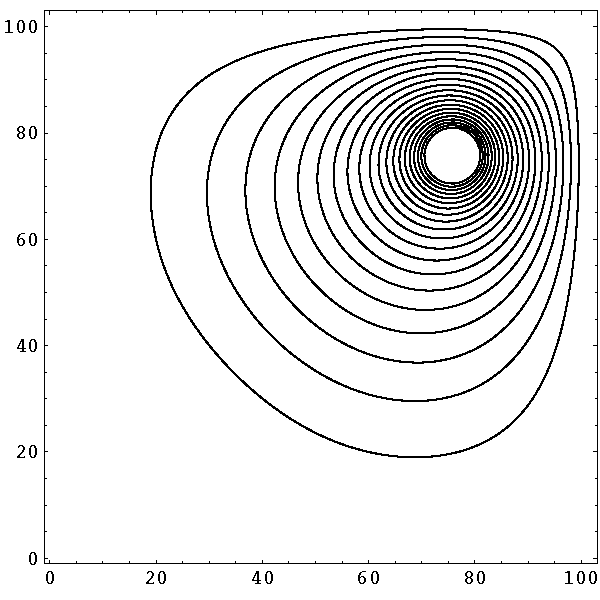
\includegraphics[width=0.8\hsize]{graphics/neilcontour}
\end{center}
\caption{Niveaulinien\label{neilcontour}}
\end{figure}
\begin{figure}
\begin{center}
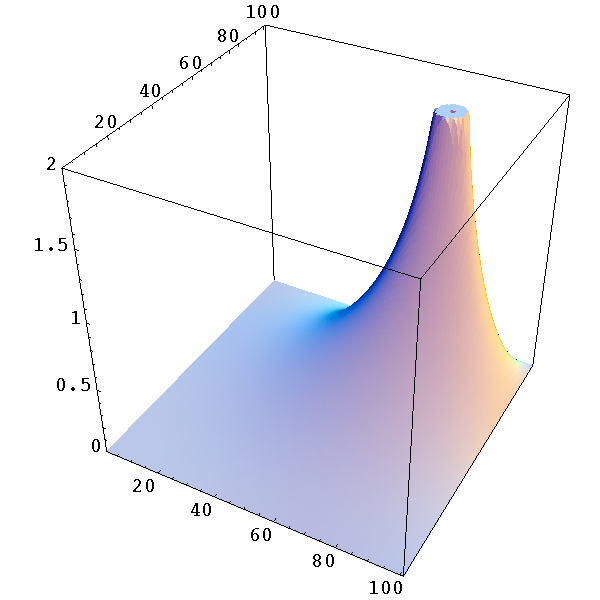
\includegraphics[width=0.8\hsize]{graphics/neilloesung}
\end{center}
\caption{Potentialfl"ache\label{neilloesung}}
\end{figure}
Dieses Beispiel illustriert, wie die Ideen dieses Kapitels verwendet werden k"onnen,
um bessere numerische L"osungen einer partiellen Differentialgleichung
zu erhalten.

{\parindent 0pt
\medskip
{\bf Aufgabe:} Eine elektrisch leitende rechteckige Platte wird am Rand und bei 
einem Punkt $x_0\in\mathbb R^2$ im Inneren mit den Polen einer Batterie verbunden. Berechnen
Sie in jedem Punkt $x$ der Platte die Spannung gegen"uber dem Rand.

\medskip
}
Das gesuchte Potential $u(x,y)$ ist eine L"osung der Gleichung
\[
\Delta u=\delta(x-x_0)
\]
mit den Randwerten
\[
u(x)=0.
\]
Direkte numerische Berechnung der L"osung w"are in der Umgebung des Punktes
$x_0$ "ausserst ungenau. Motiviert von der in diesem Kapitel entwickelten
Theorie w"ahlen wir folgendes vorgehen. Die Funktion $\sigma(x,x_0)$
ist eine harmonische Funktion mit 
\[
\Delta\sigma(x,x_0)=\delta(x-x_0)
\]
sie ist also bis auf die nicht passenden Randwerte eine L"osung.
Eine korrekte L"osung erh"alt man daher, in dem man das Randwertproblem
\begin{align*}
\Delta h(x)&=0&&x\in\Omega\\
h(x)&=-\sigma(x,x_0)&&x\in\partial\Omega
\end{align*}
l"ost, was mit g"angigen Programmen sehr effizient m"oglich ist.
Die Funktion 
\[
u(x)=\sigma(x,x_0)+h(x)
\]
ist eine L"osung. Die L"osung und die zugeh"origen Niveaulinien
sind in den Abbildungen \ref{neilloesung} und \ref{neilcontour} dargestellt.

\section{Mittelwerteigenschaft harmonischer Funktionen}
\rhead{Mittelwerteigenschaft}
Harmonische Funktionen haben eine Eigenschaft, die "uber das Maximumprinzip
f"ur elliptische Operatoren hinausgeht.
Das Maximumprinzip sagt, dass die Werte der L"osung einer homogenen
elliptischen partiellen Differentialgleichung zwischen den
Extremwerten auf dem Rand liegen.
Die Mittelwerteigenschaft sagt dar"uber hinaus, dass die Funktionswerte
(geeignete) Mittelwerte der Randwerte sind.

\subsection{Mittelwerteigenschaft}
In diesem Abschnitt wollen wir illustrieren, dass
Werte von harmonischen Funktionen in einem Punkt
Mittelwerte der Funktionswerte auf einer Kugel um den gegebenen Punkt sind.

\begin{satz}[Mittelwerteigenschaft]
Sei $u$ eine harmonische Funktion im Gebiet $\Omega$ und $x_0\in\Omega$.
%\marginpar{\tiny Mittelwerteigenschaft harmonischer Funktionen}
Sei $r$ so klein, dass die Kugel mit Radius $r$ um den Punkt $x_0$
ebenfalls in $\Omega$ enthalten ist. Dann gilt
\[
u(0)=\frac1{\mu(S^{n-1}_r)}\int_{S^{n-1}_r}u(x)\,d\mu(x).
\]
\end{satz}
\begin{proof}[Beweis]
Wir k"onnen ohne Beschr"ankung der Allgemeinheit annehmen, dass $x_0=0$.
Wegen 
\[
\Delta u=\operatorname{div}\operatorname{grad}u
\]
folgt aus dem Satz von Gauss
\begin{align*}
0&=\int_{B_r^n}\Delta u\,d\mu(x)
\\
&=\int_{B_r^n}\operatorname{div}\operatorname{grad}u\,d\mu(x)
\\
&=\int_{S_r^{n-1}} \operatorname{grad}u\cdot dn
\end{align*}
Andererseits ist 
\begin{align*}
\frac{d}{dr}\frac{1}{\mu(S_r^{n-1})}\int_{S_r^{n-1}} u(x)\,d\mu(x)
&=
\frac1{\mu(S_1^{n-1})}\frac{d}{dr}\int_{S_1^{n-1}}u(xr)\,d\mu(x)
\\
&=
\frac1{\mu(S_1^{n-1})}\int_{S_1^{n-1}}\operatorname{grad}u(xr)\cdot x
\,d\mu(x)
\\
&=
\frac1{\mu(S_1^{n-1})}\int_{S_1^{n-1}}\operatorname{grad}u(xr)\cdot dn=0
\end{align*}
Der Mittelwert h"angt also nicht vom Radius ab. Da aber wegen
der Stetigkeit von $u$ im Punkt $0$ auch
\[
\lim_{r\to 0}\frac1{S_r^{n-1}}\int_{S_r^{n-1}}u(x)\,d\mu(x)=u(0)
\]
folgt die Behauptung.
\end{proof}

Man kann die Mittelwerteigenschaft auch daf"ur verwenden, das Dirichlet-Problem
auf einem Ball zu l"osen:

\begin{satz}[Poisson-Formel]
\index{Poisson-Formel}
Sei $g$ eine stetige Funktion auf dem Rand der $n$-dimensio\-nalen
%\marginpar{\tiny Poisson-Formel}
Einheitskugel, dann ist
\[
u(x)=\begin{cases}
\displaystyle \frac{1-|x|^2}{\mu(S^{n-1})}
\int_{S^{n-1}}\frac{g(\xi)}{|x-\xi|^n}\,d\mu(\xi)&\qquad |x|<1\\
g(x)&\qquad |x|=1
\end{cases}
\]
eine harmonische Funktion mit Randwerten $u_{|S_1^{n-1}}=g$.
\end{satz}

\subsection{Maximumprinzip und Mittelwerteigeschaft}
\rhead{Maximumprinzip}
\index{Maximumprinzip}
\begin{satz}[Maximumprinzip]Ist die Funktion $u$ auf dem Gebiet
%\marginpar{\tiny Maximumprinzip f"ur harmonische Funktionen}
$\Omega$ harmonisch, und nimmt sie in einem inneren Punkt $x\in\Omega$
ein Maximum an, dann ist $u$ konstant.
\end{satz}

\begin{proof}[Beweis]
Sei $x_0\in\Omega$ der innere Punkt, in dem die Funktion $u$
ihr Maximum annimmt. Dann ist auch eine kleine Kugel mit Radius
$r$ in $\Omega$ enthalten, deren Oberfl"ache wir mit $K_r$
bezeichen. Falls $u$ nicht konstant ist, gibt
es eine Zahl $\varepsilon > 0$ und 
ein Teilgebiet $S\subset K_r$ nicht verschwindenden Volumnes $\mu(S)$,
auf welchem die Funktionswerte
mindestens $\varepsilon$ kleiner sind, also
\[
u(x)<u(x_0)-\varepsilon\quad\text{f"ur $x\in S$}
\]
Der Funktionswert in $x_0$ ist aber der Mittelwert der Funktionswerte
"uber die Kugeloberfl"ache, also
\begin{align*}
u(x_0)
&=
\frac1{\mu(K_r)}\int_{K_r}u(x)\,d\mu(x)
\\
&=\frac1{\mu(K_r)}\int_Su(x)\,d\mu(x)+\frac1{\mu(K_r)}\int_{K_r\setminus S}u(x)\,d\mu(x)
\\
&\le \frac1{\mu(K_r)}\int_S u(x_0)\,d\mu(x)+\frac1{\mu(K_r)}\int_{K_r\setminus S}u(x_0)-\varepsilon\,d\mu(x)
\\
&\le \frac1{\mu(K_r)}u(x_0)\mu(S)+\frac1{\mu(K_r)}(u(x_0)-\varepsilon)\mu(K_r\setminus S)
\\
&=
u(x_0)-\varepsilon\frac{\mu(S)}{\mu(K_r)}<u(x_0)
\end{align*}
Ein solches Teilgebiet $S$ kann es daher nicht geben, der Funktionswert
von $u$ muss auf der ganzen Kugel identisch sein.
\end{proof}

Aus dem Maximum-Prinzip folgt auch, dass eine beliebige Funktion, die
%\marginpar{\tiny Funktionen mit Mittelwerteigenschaft sind harmonisch}
die Mittelwerteigenschaft hat, auch harmonisch ist. Ist $u$ ein
Funktion, die die Mittelwerteigenschaft hat, dann kann man mit der
Poisson-Formel eine Funktion $v$ innerhalb eines Balles konstruieren,
welche auf der Oberfl"ache des Balles mit $u$ "ubereinstimmt.
Die Differenz ist dann eine Funktion, die ebenfalls die Mittelwerteigenschaft
hat, aber auch auf dem Rand des Balles verschwindet. Da die Differenz
nach dem Maximumprinzip
im Inneren das Balles nicht gr"osser sein kann als auf dem Rand,
muss $u=v$ sein. Da $v$ harmonisch ist, ist auch $u$ harmonisch.

Die Analogie zum eindimensionalen Fall ist ebenfalls durchf"uhrbar.
%\marginpar{\tiny Maximumprinzip gilt auch im eindimensionalen Musterproblem}
Ist $u$ eine Funktion von einer Variablen mit $u''=0$, dann ist
$u$ linear, also $u(x)=ax+b$. Hat $u(x)$ ein Maximum im Inneren
des Definitionsbereichs, folgt $u'(x)=a=0$, also ist $u(x)=b$ konstant.

\section{Verallgemeinerungen}
\rhead{Verallgemeinerungen}
Die in diesem Kapitel gefundenen Methoden k"onnen in verschiedene Richtungen
verallgemeinert werden.
\subsection{Neumann-Randbedingungen}
\index{Neumann-Randbedingungen}
Das Dirichlet-Problem wurde mit Hilfe einer Greenschen Funktion $G(x,\xi)$
gel"ost, welche als Funktion von $x$ die Randbedingung
\[
G(x,\xi)=0\quad\forall x\in\partial\Omega
\]
erf"ullt.
Verwendet man stattdessen eine Greensche Funktion, welche die
%\marginpar{\tiny Greensche Funktion f"ur Neumann-Randbedingungen}
Neumann-Randbedingungen
\[
\frac{\partial}{\partial n}G(x,\xi)=0\quad\forall x\in\partial\Omega
\]
erf"ullt, bleibt im Beweis von \ref{dirichletloesung}
die Formel
\begin{align*}
u(x)&=\int_{\Omega}G(x,\xi)f(\xi)\,d\mu(\xi)+\int_{\partial\Omega}G(x,\xi)\operatorname{grad}u(\xi)\cdot dn
\end{align*}
stehen. F"ur Neumann-Randbedingungen $\partial_n u=g$ kann man dies ersetzen
durch
\begin{align*}
u(x)&=\int_{\Omega}G(x,\xi)f(\xi)\,d\mu(\xi)+\int_{\partial\Omega}G(x,\xi)g(\xi)\,d\mu(\xi)
\end{align*}
Auch f"ur Neumann-Randbedingungen gibt es also eine Greensche Funktion, welche
das Problem f"ur beliebige Randwerte l"ost.

\subsection{Allgemeinere Operatoren}
Die Greensche Funktion kann unter gewissen Voraussetzungen
von die Koeffizienten auch f"ur beliebige elliptische Operatoren
\[
Lu=\biggl(\sum_{i,j}a_{ij}\frac{\partial^2}{\partial x_i\partial x_j}
+\sum_ib_i\frac{\partial}{\partial x_i} +c\biggr)u
\]
zweiter Ordnung konstruiert werden.

\subsection{Abstrakte Formulierung}
Das in diesem Kapitel erreichte kann auch wie folgt formuliert werden.
Gegeben war elliptischen Operator $L$ und ein weiterer Operator $B$,
der aus der Funktion $u$ die relevanten Randwerte ermittelte. $Bu$
ist ein Funktion auf dem Rand $\partial \Omega$ des Gebietes. 
Das Problem
\begin{align*}
Lu&=f(x)&&x\in\Omega
\\
Bu&=g(x)&&x\in\partial\Omega
\end{align*}
konnte mit Hilfe einer Integralformel
\[
u(x)=\int_\Omega G(x,\xi)f(\xi)\,d\mu(\xi)+\int_{\partial \Omega}K(x,\xi)g(\xi)\,d\mu(\xi)
\]
gel"ost werden.
Die Funktionen $G$ und $K$ erm"oglichen also, die Operatoren $L$ und $B$
zu invertieren.

\section{Zusammenfassung: das Wichtigste in K"urze}
\begin{enumerate}
\item Die Differentialgleichung $\Delta u=f$ ist der prototypische
elliptische partielle Differentialgleichung.
\item L"osungen homogener elliptischer partieller Differentialgleichungen,
insbesondere auch von $\Delta u=0$, erf"ullen das Maximumprinzip:
Maximum und Minimum von $u$ liegen auf dem Rand des Gebietes.
\item Die L"osung einer elliptischen Differentialgleichung auf einem
beschr"ankten Gebiet mit Randwertvorgaben entlang des gesamten Randes
ist eindeutig.
\item Eine gut gestellte elliptische partielle Differentialgleichung hat
eine Greensche Funktion, d.~h.~eine L"osung der Differentialgleichung
$\Delta G(x,\xi)=\delta_\xi$ f"ur jeden Punkt $\xi\in\Omega$.
\item Mit Hilfe der Greenschen Funktion l"asst sich die L"osung
der Differentialgleichung mittels eines Integrals "uber das Gebiet
berechnen.
\item Harmonische Funktionen sind L"osungen der Gleichung $\Delta u=0$.
\item Harmonische Funktionen haben die Mittelwerteigenschaft: Funktionswerte
in einem Punkt sind Mittelwerte der Funktionswerte auf einer Kugel
um den Punkt.
\end{enumerate}


